% This needs jlcode.sty, for Julia code.
% I put it into a texmf subdirectry and run "export TEXINPUTS=.:./texmf/:".
% Build with pdflatex distributions.tex, or latexmk -pdf distributions.tex.
\documentclass{article}
\usepackage{hyperref}
\usepackage{jlcode} % https://github.com/wg030/jlcode
\usepackage{listings}
\usepackage{amsfonts}
\usepackage{mathtools}
%\usepackage{sourcecodepro}
% \usepackage[usenames,dvipsnames]{xcolor}
\usepackage[T1]{fontenc}
\usepackage{xspace}
\usepackage{bookman}
\usepackage{tikz}

\newcommand{\gsmp}{\textsc{gsmp}\xspace}
\newcommand{\gspn}{\textsc{gspn}\xspace}


\title{Sampling Distributions for GSMP in Julia}
\author{Andrew Dolgert}
\begin{document}
\maketitle

\tableofcontents

\section{Introduction}

Our goal is to write continuous-time simulation of a generalized semi-Markov process (\gsmp) or generalized stochastic Petri net (\gspn). They use the same samplers, as do chemical simulations, queuing theory, vector addition systems, and so on.  There are many ways to sample these distributions, and they involve different mathematical manipulations of those distributions. This document looks at the functions defined by Julia for manipulating distributions in order to figure out how to write samplers in Julia, so it's going to connect the math with the code, asking how to be efficient within the Julia framework.

Because manipulating distributions for no reason is tedious, let's motivate ourselves with the goal. All of the kinds of simulation above have a common way to select the time for the next event. Anderson and Kurtz have a unified view which they call \emph{competing processes}. In the language of \gsmp, it's called \emph{competing clocks}, and I'll use the term ``clock'' in the code.

These continuous-time simulations stop at time points $T_i$, indexed by $i$. At any time point, the next time point is determined by competion among a finite set of clocks. Each clock has an enabling time, which is one of the past $T_i$ time points, and each clock has a probability density that determines the next time it would fire. The first job of the sampler is to choose the next state and time among the currently-enabled clocks. The second job of the sampler is to account for clocks that are disabled and enabled at that time point in order to sample the next one, and to do it efficiently.

\section{Notation for Distributions}\label{sec:notation}%

We need to use some accepted notation for a statistical distribution. Let's choose some variable names to use.

A \emph{cumulative distribution} is the probability of an event before a given time. The random variate is $T$ and $t$ is a parameter. $P$ denotes a probability, and $F$ is the name we choose for a general cumulative distribution, or cdf.
\begin{equation}
  P(T \le t) = F(t)
\end{equation}
The survival is the probability an event fires after time $t$.
\begin{equation}
  P(T > t) = G(t) = 1 - F(t)
\end{equation}
The \emph{probability density function,} or pdf, is the derivative of the cumulative distribution.
\begin{equation}
  f(t) = dF(t)/dt
\end{equation}
% This distribution can combine continuous and point distributions.
% \begin{equation}
%   F(t) = F'(t) + \sum_i f_i\delta(t-t_i)
% \end{equation}
The \emph{hazard rate} is the probability per unit time of an event, given that it has not yet fired.
\begin{equation}
\lim_{\delta t\rightarrow 0} P(t < T\le t + \delta t) = \lambda(t)
\end{equation}
Every continuous distribution can be written in terms of the hazard rate.
\begin{equation}
F(t) = 1 - e^{-\int_0^t\lambda(s)ds}
\end{equation}
This means the pdf is also a function of hazard rate.
\begin{equation}
f(t) = \lambda(t)e^{-\int_0^t\lambda(s)ds}
\end{equation}
The survival, in terms of the hazard rate, is one term.
\begin{equation}
S(t)=e^{-\int_0^t\lambda(s)ds}
\end{equation}
Because the survival has this form, where it's an integral in the exponential, we can think of intermediate waypoints in time.
\begin{equation}
	S(t)=e^{-\int_0^{t_1}\lambda(s)ds}e^{-\int_{t_1}^t\lambda(s)ds}
\end{equation}
Each of the terms is a conditional survival, written $S(t_1,t_2)$. In other words,
\begin{equation}
	S(t) = S(0, t) = S(0, t_1)S(t_1,t),
\end{equation}
so people say the conditional survival is multiplicative. Going back to the powerful probability language the conditional survival can be written in terms of the marginal survival.
\begin{equation}
	P(T>t|T>t_1) = \frac{P(T>t)}{P(T>t_1)}.
\end{equation}
Multiplying both sides shows that conditional survival is multiplicative.
\begin{equation}
	P(T>t)=P(T>t_1)P(T>t|T>t_1)
\end{equation}
Another way to look at a conditional survival is in the cdf space, where it becomes a fraction.
\begin{equation}
	S(t_1,t) = \frac{S(t)}{S(t_1)} = \frac{1-F(t)}{1-F(t_1)}
\end{equation}
Writing the survival in terms of the hazard also makes it easier to see how it relates to the pdf.
\begin{equation}
	f(t)=-\frac{d}{dt}S(t)
\end{equation}
The log of the survival is called the integrated hazard.
\begin{equation}
\ln S(t) = -\int_0^t\lambda(s)ds = -\Lambda(t)
\end{equation}
You can get the hazard directly from survival and the pdf.
\begin{equation}
	\lambda(t) = \frac{f(t)}{S(t)}
\end{equation}
Rearranging slightly shows us a form we'll see later, $f(t)=\lambda(t)S(t)$.

What if we had a distribution described by $\lambda(t)$ and wanted to define a new distribution that started later. For instance, a Gamma distribution fits our data, but only if it starts after $t_0=0.1$? For such a distribution, the new survival would be
\begin{equation}
	S'(t)=e^{-\int_{t_0}^{t_0+t}\lambda(s)ds} = \frac{S(t_0,t_0+t)}{S(0, t_0)}.
\end{equation}
An even easier way to think about how the distribution changes is to consider changes not to the exponential but to the integral inside the exponential.
\begin{equation}
	\Lambda'(t) = \int_{t_0}^{t_0+t}\lambda(s)ds = \int_0^{t_0+t}\lambda(s)ds - \int_0^{t_0}\lambda(s)ds = \Lambda(t_0+t) - \Lambda(t_0)
\end{equation}
If, for some reason, we need to think about shifting distributions, and if we can work in this space of survivals and integrated hazards, then there are concise ways to recalculate a shifted distribution from its original form.


\section{Julia Distributions}\label{sec:juliadist}
Julia has a \texttt{Distributions.jl} library that contains univariate distributions, which are what we want. Let's walk through the functions this package offers for working with those distributions. We can write each function's mathematical equivalent.

\subsection{Parameters}
Julia has one function to retrieve all parameters of a distribution and a few functions that are specific to common parameters.

\begin{itemize}
	\item \texttt{params(d::UnivariateDistribution)}---Gets all parameters for a distribution.
	\item \texttt{scale(d::UnivariateDistribution)}---If the distribution has a parameter $\theta$ and is written as $f(t/\theta)$, then $\theta$ is the scale.
	\item \texttt{rate(d::UnivariateDistribution)}---If the distribution has a parameter $\beta$ and is written as $f(\beta t)$, then $\beta$ is the rate. We see that $\beta\theta = 1$.
	\item \texttt{location(d::UnivariateDistribution)}---If the distribution has a parameter $\mu$ and is written as $f(t-\mu)$, then $\mu$ is the location. This will be important for re-sampling distributions which failed to fire.
	\item \texttt{shape(d::UnivariateDistribution)}---The shape is often a power, $k$, of $t^k$ in the pdf.
\end{itemize}

\subsection{Probability Evaluation}

\begin{table}
\begin{tabular}{|lll|} \hline
	Julia Function & Equation & Statistics name \\ \hline
	\texttt{ccdf} & $S(x) = e^{-\int^x\lambda(s)ds}$ & Survival \\
	\texttt{cdf} & $F(x) = 1 - S(x) = 1-e^{-\int^x\lambda(s)ds}$ & Cumulative distribution function \\
	\texttt{pdf} & $f(x) = \lambda(x)e^{-\int^x\lambda(s)ds}$ & Probability density function \\
	\texttt{logpdf} & $\ln\:f(x)$ & Log probability density \\
	\texttt{logcdf} & $\ln\:F(x)$ & \\
	\texttt{logdiffcdf} & $\ln\left(F(x_2)-F(x_1)\right)$ & \\
	\texttt{logccdf} & $-\int^x\lambda(s)ds$ & Integrated hazard (negated) \\
	\texttt{quantile} & $y = F^{-1}(x)$ & Inverse cumulative distribution function \\
	\texttt{cquantile} & $y = F^{-1}(1-x)$ so $x = S(y)$ & Inverse Survival \\
	\texttt{invlogcdf} & $x = \ln\:F(y)$ so $e^x = F(y)$ & \\
	\texttt{invlogccdf} & $x = -\int_0^y\lambda(s)ds$ & Inverse negative integrated hazard \\ \hline
\end{tabular}
\caption{This translates between Julia functions and hazard-based notation. We can use this to find
the shortest path to our calculation in code.\label{julia-translation}}
\end{table}

Later we will use two pairs of functions from \texttt{Distributions.jl} to implement Next Reaction method. The first pair is the survival and its inverse: \texttt{ccdf()} and \texttt{cquantile()}. You can see in Tab.~\ref{julia-translation} that these are inverses of each other. The second pair is the same, but in the log-space.

\texttt{invlogccdf(d::UnivariateDistribution, x::Real)} can be translated into
\begin{equation}
e^x = G(y) = e^{-\int_0^y\lambda(s)ds}.
\end{equation}
That means this function is the inverse of the integrated hazard.
\begin{equation}
x = \Lambda(y)
\end{equation}
In this package, the integrated hazard is the negative of \texttt{logccdf}.


\section{Next Reaction for Non-Markov Processes}\label{sec:nextreaction}

Many of the calculations below rely on fluency with shifted distributions. Shifted distributions are the basis of the Next Reaction method and Modified Next Reaction method, so we will derive those methods here, but the further goal is to be comfortable with calculation of shifted distributions.

While the final code will rarely use sampling by inversion, it helps to start with in order to work out concepts. Using the notation from Sec.~\ref{sec:notation}, we write sampling by inversion as two steps. First, draw a random number from $0\le U<1$. Then invert the cdf to find the sampled relative time $t$.
\begin{equation}
	U = F(t)
\end{equation}
However, since the survival is one minus the cdf, we can also write this as
\begin{equation}
	U = S(t)\label{eqn:basesample}
\end{equation}
with the same resulting density function of the sampled random variable.

Because simulations move through time and transitions are enabled and disabled, we have to agree on notation for time relative to the start of a transition and how it relates to absolute time within the simulation.

\begin{itemize}
\item $t$---Time relative to the zero-point of the distribution, as implemented in \texttt{Distributions.jl}. If you look up a gamma distribution in Wikipedia, it is relative to some implied start time at $t=0$, and we denote its pdf with $f(t)$, as you saw in Sec.~\ref{sec:notation}.

\item $t_e$---Absolute time at which the transition is enabled. This acts as a location parameter for distributions. It is traditionally handled outside of the internals of any distribution because so much of sampling competing processes is about shifting the location of whole sets of distributions efficiently.

\item $t_0$---Absolute time at which to place the zero-point of the distribution. If $t_0 < t_e$, it's equivalent to saying that we are cutting off the left side of the distribution, up to $t=t_e-t_0$. If $t_0>t_e$, it's equivalent to saying the transition cannot possibly fire until after time absolute time $t_0$.

\item $t_n$---We'll use this to represent some later absolute time at which the distribution changes its parameters in some way.
\end{itemize}

Let's start with the simplifying assumption that the distribution doesn't have a location shift, so $t_0=t_e$. Use Eq.~\ref{eqn:basesample} to write sampling in absolute time.
\begin{equation}
	u = S(\tau - t_e)
\end{equation}
When we invert it, this is
\begin{equation}
	\tau = t_e + S^{-1}(u).
\end{equation}
Another way to write this is to expand the exponential.
\begin{equation}
u=\exp\left(-\int_{t_e}^{\tau}\lambda(s-t_e)ds\right)\label{eqn:exponentialform}
\end{equation}
This shows that there is a integration inside the exponent. We can use this in the Next Reaction scheme.

Suppose there were a time $t_e$ at which a transition was enabled. Then, at a later time, $t_n$, a change in simulation state changed the parameters of the transition. Could we figure out what the drawn time, $\tau$, would have been had we known that the parameters would change?

During the draw in Eq.~\ref{eqn:exponentialform}, the distribution we draw from is described by its hazard, $\lambda$, so let's label the initial hazard $\lambda_0$ and the subsequent hazard $\lambda_n$.
\begin{eqnarray}
	u&=&\exp\left(-\int_{t_e}^{\tau}\lambda_0(s-t_e)ds\right) \\
	&=& \exp\left(-\int_{t_e}^{t_n}\lambda_0(s-t_e)ds\right)\exp\left(-\int_{t_n}^{\tau'}\lambda_{n}(s-t_e)ds\right)\label{eqn:expequivalence}
\end{eqnarray}
We can think of the new draw, $\tau'$ as coming from the same element of the uniform random variate, $u$. Gibson and Bruck make the point that integration is a linear operator, which is what makes the separation in Eq.~\ref{eqn:expequivalence} work.

The algorithm of Gibson and Bruck starts with the draw from Eq.~\ref{eqn:exponentialform}.
\begin{enumerate}
	\item Draw an element $u$ from a uniform random variate $U$.

	\item Solve for a putative firing time $\tau$ by inverting the survival equation, Eq.~\ref{eqn:exponentialform}.

	\item If, at some later time $t_n$, there is a change to the parameters of the distribution, then calculate the conditional survival up to $t_n$ and update the element $u$.
	\begin{equation}
		u'=u\exp\left(-\int_{t_e}^{t_n}\lambda_0(s-t_e)ds\right)
	\end{equation}

	\item Since you were able to invert the survival before, you can do it again, this time with $u'$ and the updated hazard rate.
	\begin{equation}
		u'=\exp\left(-\int_{t_n}^{\tau'}\lambda_{n}(s-t_e)ds\right)
	\end{equation}
	Solving this gives for $\tau'$ gives the new draw, effectively from the old uniform variate, $u$.
\end{enumerate}

If we return to Eq.~\ref{eqn:expequivalence}, wouldn't it be easier to compute if we could take the logarithm of both sides?
\begin{equation}
	\ln u=-\int_{t_e}^{\tau}\lambda_0(s-t_e)ds = -\int_{t_e}^{t_n}\lambda_0(s-t_e)ds - \int_{t_n}^{\tau'}\lambda_{n}(s-t_e)ds\label{eqn:logequivalence}
\end{equation}
This log-space calculation is what Anderson's modified next reaction recommends. It turns out that calculations in this space are both faster and more precise for most of the distributions commonly used in simulation, such as the Exponential, Gamma, and Erlang distributions.

Now is a good time to return to the assumption that every distribution's zero-point is the same as when the transition is enabled, $t_0=t_e$. Remember that the goal of differentiating the two is to allow a subject-matter expert to declare that, for instance, a process will take at least 10~minutes and then be exponentially-distributed after that. Or, they can tell you that it looks like the last third of a Gaussian distribution. Because the Next Reaction method's central calculation is how to shift a distribution, a user-specified shift in the specification can be handled within the algorithm. When $t_0\ne t_e$, the algorithm respects the difference the first time it samples but then saves only $t_e$ for later use.

Let's walk through the cases because they clarify what we need to store within the sampler.
\begin{itemize}
	\item First time enabling the transition. Sample any way possible from $S(t_n-t_e, \tau-t_n)$, but then calculate and store $U=S(t_n-t_e, \tau-t_n)$.
	\item Enabling a transition that fired. Sample any way possible from $S(t_n-t_e, \tau-t_n)$, but then calculate and store $U=S(t_n-t_e, \tau-t_n)$.

	\item Enabling a transition that was disabled before it fired.
	\begin{itemize}
		\item General case. Sample by inversion $U=S(t_n-t_e, \tau-t_n)$.
		\item The transition is picking up where it left off. We don't have to sample because the firing time is just pushed forward. Does this happen often enough to care? If the previous distribution was $(t_e, t_n, f)$ when it was disabled at time $t_n$, we know the transition is merely shifted because, at time $t_{n+1}$, it has the form $(t_{n+1}-(t_e-t_n), t_{n+1}, f)$. In this case, $\tau' = \tau + t_{n+1}-t_n$, and there is no change to the stored $U$.
	\end{itemize}
	\item Disabling a transition that did not fire. If a transition did not fire at time $t_{n+1}$, calculate conditional survival, $S(t_n-t_e, t_{n+1}-t_e)$ and adjust the stored $U$ by dividing by the conditional survival.
	\item Disabling the transition that fired. If we adjust the conditional survival according to the formula above, it may close to zero but not equal. We need it to be $U=0$, so set that value.
\end{itemize}
From the cases above, the sampler needs to store two kinds of information.
\begin{itemize}
	\item Long-term values about all transitions. These are $U$, $t_e-t_n$, and $f$.
	\item Short-term values for currently-enabled transitions. These are $t_e$, $t_n$, $f$.
\end{itemize}

There are a couple of challenges. One is how to know when two floating-point values are equal, such as in the check that the transition is picking up where it left off. This is handled in code by calculating the machine epsilon for a floating point of the size of $t_n$. Multiply that by a small factor, such as 2 or 4, and use that as an error bound.

Another challenge is how to figure out which disabled transition is the one that fired. If the caller specifies it is disabling the transition that fired, then it's clear. If the caller doesn't specify, can we know? The transitions are in a heap where the soonest is on top. If the first transition that's disabled was the one on top and the next transition becomes the one on top, it could look like it was next to fire. We could check the times on those transitions in order to see whether the time of disabling matches the time of the top transition, but that's prone to error because it requires equality of floating-point numbers. There will definitely be some time when two numbers in a continuous time simulation are very close to each other.

On the other hand, there isn't a good way to use a Next Reaction sampler except to always choose the transition it sampled to be next. Let's store the response from the next() function and assume that's the one that fired when it gets disabled.

\section{Timing Sampling Methods}

The Next Reaction method (Gibson and Bruck) and the Modified Next Reaction method (Anderson) are essentially the same algorithm except that one samples in a linear space and one samples in a logarithmic space. Which one is better depends on the distribution we're sampling and the parameter ranges for that distribution. This section looks at tests of the distributions defined in Julia in order to classify which one goes in which category, linear or logarithmic sampling.

Below is a table that comes from a test in \texttt{test/nrmetric.jl}. The distributions come from \texttt{Distributions.jl}. Each distribution appears twice, once with default parameters and once as a truncated distribution, which is Julia's way of limiting the distribution's support so that we can sample values that are later than a given time. Each distribution is tested on 10,000 values. The table will have the following values.

\begin{enumerate}
	\item The space for the test, which is linear or logarithmic.

	\item Error, as the log base-10 of the maximum error after sampling a survival and then inverting that back to get the sample. When the number is -16, that means the error is $10^{-16}$.

	\item Average error in log base-10, which is the trimmed mean over all runs of the error in the previous column.

	\item Forward timing in seconds. For the linear space, this is the time to perform the \texttt{ccdf} call. For the logarithmic space, this is the time to perform the \texttt{logccdf} call, both 10,000 times. A time of 6e-4 seconds means each iteration took, on average, 6e-8 seconds.

	\item Backward timing in seconds. For the linear space, this is the time to perform the \texttt{cquantile} call. For the logarithmic space, this is the time to perform the \texttt{invlogccdf} call, both 10,000 times.
\end{enumerate}

\pagebreak
\begin{tabular}{|llrrrrr|} \hline
& Space & $\mbox{log}_{10}|\epsilon|_1$ & $\mbox{log}_{10}\langle\epsilon\rangle$ & forward [s] & backward [s] & both [s]\\ \hline
\multicolumn{7}{|l|}{Arcsine\{Float64\}(a=0.0, b=1.0)}\\ \hline
& Linear & -12.7 & {\color{blue}-16.5} & {\color{blue}8.34e-05} & {\color{blue}7.52e-05} & {\color{blue}1.59e-04}\\
& Log & {\color{blue}-15.4} & -16.3 & 1.99e-04 & 9.08e-05 & 2.90e-04\\
\hline
\multicolumn{7}{|l|}{Truncated(Arcsine\{Float64\}(a=0.0, b=1.0); lower=0.01, upper=Inf)}\\ \hline
& Linear & -12.9 & -16.2 & {\color{blue}1.05e-04} & {\color{blue}6.43e-05} & {\color{blue}1.69e-04}\\
& Log & {\color{blue}-15.4} & {\color{blue}-16.3} & 5.48e-04 & 1.54e-04 & 7.01e-04\\
\hline
\multicolumn{7}{|l|}{BetaPrime\{Float64\}($\alpha$=1.0, $\beta$=1.0)}\\ \hline
& Linear & {\color{blue}-15.7} & {\color{blue}-16.8} & {\color{blue}5.40e-04} & {\color{blue}2.52e-03} & {\color{blue}3.06e-03}\\
& Log & -13.9 & -15.0 & 7.25e-04 & 3.41e-03 & 4.13e-03\\
\hline
\multicolumn{7}{|l|}{Truncated(BetaPrime\{Float64\}($\alpha$=1.0, $\beta$=1.0); lower=0.01, upper=Inf)}\\ \hline
& Linear & {\color{blue}-15.6} & {\color{blue}-16.4} & {\color{blue}5.73e-04} & {\color{blue}2.52e-03} & {\color{blue}3.09e-03}\\
& Log & -13.7 & -14.9 & 8.31e-04 & 2.64e-03 & 3.47e-03\\
\hline
\multicolumn{7}{|l|}{Biweight\{Float64\}($\mu$=0.0, $\sigma$=1.0)}\\ \hline
& Linear & {\color{blue}-13.4} & {\color{blue}-14.2} & {\color{blue}7.00e-06} & {\color{blue}7.92e-04} & {\color{blue}7.99e-04}\\
& Log & -11.1 & -13.9 & 1.14e-04 & 4.20e-03 & 4.31e-03\\
\hline
\multicolumn{7}{|l|}{Truncated(Biweight\{Float64\}($\mu$=0.0, $\sigma$=1.0); lower=0.01, upper=Inf)}\\ \hline
& Linear & {\color{blue}-13.0} & {\color{blue}-13.6} & {\color{blue}3.30e-05} & {\color{blue}7.99e-04} & {\color{blue}8.32e-04}\\
& Log & -11.1 & -13.3 & 2.59e-04 & 8.85e-04 & 1.14e-03\\
\hline
\multicolumn{7}{|l|}{Beta\{Float64\}($\alpha$=1.0, $\beta$=1.0)}\\ \hline
& Linear & -16.0 & -16.9 & {\color{blue}5.25e-04} & {\color{blue}2.51e-03} & {\color{blue}3.04e-03}\\
& Log & {\color{blue}-16.0} & {\color{blue}-17.1} & 6.72e-04 & 3.41e-03 & 4.08e-03\\
\hline
\multicolumn{7}{|l|}{Truncated(Beta\{Float64\}($\alpha$=1.0, $\beta$=1.0); lower=0.01, upper=Inf)}\\ \hline
& Linear & -15.7 & -16.5 & {\color{blue}5.50e-04} & 2.51e-03 & {\color{blue}3.06e-03}\\
& Log & {\color{blue}-15.7} & {\color{blue}-16.6} & 8.00e-04 & {\color{blue}2.41e-03} & 3.21e-03\\
\hline
\multicolumn{7}{|l|}{Cauchy\{Float64\}($\mu$=0.0, $\sigma$=1.0)}\\ \hline
& Linear & {\color{blue}-16.0} & {\color{blue}-17.5} & {\color{blue}7.09e-05} & {\color{blue}1.37e-04} & {\color{blue}2.08e-04}\\
& Log & -13.5 & -14.5 & 3.41e-04 & 1.65e-04 & 5.06e-04\\
\hline
\multicolumn{7}{|l|}{Truncated(Cauchy\{Float64\}($\mu$=0.0, $\sigma$=1.0); lower=0.01, upper=Inf)}\\ \hline
& Linear & {\color{blue}-15.5} & {\color{blue}-16.2} & {\color{blue}8.79e-05} & {\color{blue}1.34e-04} & {\color{blue}2.22e-04}\\
& Log & -13.3 & -14.4 & 4.18e-04 & 1.74e-04 & 5.93e-04\\
\hline
\multicolumn{7}{|l|}{Cosine\{Float64\}($\mu$=0.0, $\sigma$=1.0)}\\ \hline
& Linear & {\color{blue}-10.8} & {\color{blue}-11.3} & {\color{blue}8.26e-05} & {\color{blue}8.42e-03} & {\color{blue}8.50e-03}\\
& Log & -5.4 & -11.1 & 2.43e-04 & 8.72e-03 & 8.96e-03\\
\hline
\multicolumn{7}{|l|}{Truncated(Cosine\{Float64\}($\mu$=0.0, $\sigma$=1.0); lower=0.01, upper=Inf)}\\ \hline
& Linear & {\color{blue}-10.5} & -11.0 & {\color{blue}9.33e-05} & 8.35e-03 & {\color{blue}8.44e-03}\\
& Log & -5.4 & {\color{blue}-11.1} & 3.68e-04 & {\color{blue}8.15e-03} & 8.52e-03\\
\hline
\end{tabular}

\pagebreak
\begin{tabular}{|llrrrrr|} \hline
& Space & $\mbox{log}_{10}|\epsilon|_1$ & $\mbox{log}_{10}\langle\epsilon\rangle$ & forward [s] & backward [s] & both [s]\\ \hline
\multicolumn{7}{|l|}{Gumbel\{Float64\}($\mu$=0.0, $\theta$=1.0)}\\ \hline
& Linear & {\color{blue}-15.8} & {\color{blue}-16.9} & {\color{blue}9.53e-05} & 3.01e-04 & {\color{blue}3.96e-04}\\
& Log & Inf & Inf & 3.72e-04 & {\color{blue}1.51e-04} & 5.23e-04\\
\hline
\multicolumn{7}{|l|}{InverseGamma\{Float64\}(
invd: Gamma\{Float64\}($\alpha$=1.0, $\theta$=1.0)
$\theta$: 1.0
)
}\\ \hline
& Linear & {\color{blue}-15.5} & {\color{blue}-16.8} & {\color{blue}9.97e-04} & {\color{blue}2.79e-03} & {\color{blue}3.78e-03}\\
& Log & -3.0 & -15.2 & 2.56e-03 & 5.18e-03 & 7.74e-03\\
\hline
\multicolumn{7}{|l|}{InverseGaussian\{Float64\}($\mu$=1.0, $\lambda$=1.0)}\\ \hline
& Linear & {\color{blue}-15.3} & {\color{blue}-16.2} & {\color{blue}4.99e-04} & {\color{blue}3.58e-03} & {\color{blue}4.07e-03}\\
& Log & -13.3 & -14.6 & 6.26e-04 & 1.35e-02 & 1.41e-02\\
\hline
\multicolumn{7}{|l|}{JohnsonSU\{Int64\}($\xi$=0, $\lambda$=1, $\gamma$=0, $\delta$=1)}\\ \hline
& Linear & {\color{blue}-15.4} & {\color{blue}-16.6} & {\color{blue}2.35e-04} & 3.82e-04 & {\color{blue}6.18e-04}\\
& Log & -13.8 & -14.9 & 6.72e-04 & {\color{blue}2.97e-04} & 9.68e-04\\
\hline
\multicolumn{7}{|l|}{Kolmogorov()}\\ \hline
& Linear & {\color{blue}-15.3} & -16.4 & {\color{blue}9.46e-05} & {\color{blue}9.94e-03} & {\color{blue}1.00e-02}\\
& Log & -0.8 & {\color{blue}-Inf} & 2.12e-04 & 1.09e-01 & 1.09e-01\\
\hline
\multicolumn{7}{|l|}{Kumaraswamy\{Float64\}(a=1.0, b=1.0)}\\ \hline
& Linear & {\color{blue}-16.3} & {\color{blue}-16.9} & {\color{blue}7.98e-05} & {\color{blue}7.99e-05} & {\color{blue}1.60e-04}\\
& Log & -16.0 & -16.9 & 1.14e-04 & 1.20e-04 & 2.34e-04\\
\hline
\multicolumn{7}{|l|}{Laplace\{Float64\}($\mu$=0.0, $\theta$=1.0)}\\ \hline
& Linear & {\color{blue}-16.6} & {\color{blue}-Inf} & {\color{blue}5.03e-05} & 1.70e-04 & 2.21e-04\\
& Log & -11.4 & -14.1 & 8.91e-05 & {\color{blue}6.55e-05} & {\color{blue}1.55e-04}\\
\hline
\multicolumn{7}{|l|}{Levy\{Float64\}($\mu$=0.0, $\sigma$=1.0)}\\ \hline
& Linear & {\color{blue}-15.2} & {\color{blue}-16.5} & {\color{blue}7.72e-05} & {\color{blue}8.65e-05} & {\color{blue}1.64e-04}\\
& Log & -1.9 & -14.8 & 3.74e-04 & 1.48e-04 & 5.22e-04\\
\hline
\multicolumn{7}{|l|}{Lindley\{Float64\}($\theta$=1.0)}\\ \hline
& Linear & {\color{blue}-15.4} & {\color{blue}-16.3} & {\color{blue}4.56e-05} & {\color{blue}1.51e-03} & {\color{blue}1.56e-03}\\
& Log & -12.7 & -14.3 & 1.04e-04 & 1.55e-03 & 1.66e-03\\
\hline
\multicolumn{7}{|l|}{Logistic\{Float64\}($\mu$=0.0, $\theta$=1.0)}\\ \hline
& Linear & {\color{blue}-16.0} & -17.2 & {\color{blue}5.38e-05} & 1.96e-04 & {\color{blue}2.50e-04}\\
& Log & -14.8 & {\color{blue}-17.9} & 2.52e-04 & {\color{blue}1.15e-04} & 3.66e-04\\
\hline
\multicolumn{7}{|l|}{LogitNormal\{Float64\}($\mu$=0.0, $\sigma$=1.0)}\\ \hline
& Linear & -15.4 & -16.4 & {\color{blue}1.74e-04} & {\color{blue}1.92e-04} & {\color{blue}3.66e-04}\\
& Log & {\color{blue}-15.7} & {\color{blue}-16.6} & 4.65e-04 & 2.54e-04 & 7.19e-04\\
\hline
\multicolumn{7}{|l|}{LogNormal\{Float64\}($\mu$=0.0, $\sigma$=1.0)}\\ \hline
& Linear & {\color{blue}-15.4} & {\color{blue}-16.6} & {\color{blue}1.92e-04} & {\color{blue}1.69e-04} & {\color{blue}3.61e-04}\\
& Log & -13.8 & -15.0 & 3.82e-04 & 1.93e-04 & 5.75e-04\\
\hline
\end{tabular}

\pagebreak
\begin{tabular}{|llrrrrr|} \hline
& Space & $\mbox{log}_{10}|\epsilon|_1$ & $\mbox{log}_{10}\langle\epsilon\rangle$ & forward [s] & backward [s] & both [s]\\ \hline
\multicolumn{7}{|l|}{Normal\{Float64\}($\mu$=0.0, $\sigma$=1.0)}\\ \hline
& Linear & {\color{blue}-15.5} & {\color{blue}-16.7} & {\color{blue}9.80e-07} & {\color{blue}1.43e-06} & {\color{blue}2.41e-06}\\
& Log & -14.4 & -15.3 & 4.79e-06 & 2.16e-06 & 6.95e-06\\
\hline
\multicolumn{7}{|l|}{NormalCanon\{Float64\}($\eta$=0.0, $\lambda$=1.0, $\mu$=0.0)}\\ \hline
& Linear & {\color{blue}-15.5} & {\color{blue}-16.7} & {\color{blue}8.40e-07} & {\color{blue}1.47e-06} & {\color{blue}2.31e-06}\\
& Log & -14.4 & -15.3 & 3.02e-06 & 2.26e-06 & 5.28e-06\\
\hline
\multicolumn{7}{|l|}{Pareto\{Float64\}($\alpha$=1.0, $\theta$=1.0)}\\ \hline
& Linear & {\color{blue}-16.0} & {\color{blue}-19.1} & {\color{blue}4.80e-07} & {\color{blue}5.10e-07} & {\color{blue}9.90e-07}\\
& Log & -14.1 & -15.1 & 2.05e-06 & 9.00e-07 & 2.95e-06\\
\hline
\multicolumn{7}{|l|}{PGeneralizedGaussian\{Float64\}($\mu$=0.0, $\alpha$=1.4142135623730951, p=2.0)}\\ \hline
& Linear & {\color{blue}-16.0} & {\color{blue}-16.9} & {\color{blue}2.44e-06} & {\color{blue}2.30e-05} & {\color{blue}2.54e-05}\\
& Log & Inf & Inf & 5.17e-06 & 3.10e-05 & 3.62e-05\\
\hline
\multicolumn{7}{|l|}{Rayleigh\{Float64\}($\sigma$=1.0)}\\ \hline
& Linear & {\color{blue}-16.0} & {\color{blue}-16.8} & 5.00e-07 & 1.76e-06 & 2.26e-06\\
& Log & Inf & Inf & {\color{blue}4.30e-07} & {\color{blue}1.60e-06} & {\color{blue}2.03e-06}\\
\hline
\multicolumn{7}{|l|}{Rician\{Float64\}($\nu$=0.0, $\sigma$=1.0)}\\ \hline
& Linear & {\color{blue}-15.6} & {\color{blue}-16.5} & 1.19e-05 & {\color{blue}7.51e-05} & {\color{blue}8.70e-05}\\
& Log & Inf & Inf & {\color{blue}1.09e-05} & 3.98e-04 & 4.09e-04\\
\hline
\multicolumn{7}{|l|}{SkewedExponentialPower\{Rational\{Int64\}\}($\mu$=0//1, $\sigma$=1//1, p=2//1, $\alpha$=1//2)}\\ \hline
& Linear & {\color{blue}-16.0} & {\color{blue}-16.9} & {\color{blue}5.02e-06} & {\color{blue}2.51e-05} & {\color{blue}3.02e-05}\\
& Log & Inf & Inf & 7.83e-06 & 3.35e-05 & 4.13e-05\\
\hline
\multicolumn{7}{|l|}{SymTriangularDist\{Float64\}($\mu$=0.0, $\sigma$=1.0)}\\ \hline
& Linear & -16.0 & {\color{blue}-17.0} & {\color{blue}1.60e-07} & {\color{blue}6.00e-07} & {\color{blue}7.60e-07}\\
& Log & {\color{blue}-16.0} & -16.8 & 3.64e-06 & 8.20e-07 & 4.46e-06\\
\hline
\multicolumn{7}{|l|}{Triweight\{Float64\}($\mu$=0.0, $\sigma$=1.0)}\\ \hline
& Linear & {\color{blue}-15.2} & {\color{blue}-16.0} & {\color{blue}5.00e-07} & {\color{blue}9.57e-06} & {\color{blue}1.01e-05}\\
& Log & -11.3 & -15.7 & 1.46e-06 & 5.65e-05 & 5.79e-05\\
\hline
\multicolumn{7}{|l|}{Uniform\{Float64\}(a=0.0, b=1.0)}\\ \hline
& Linear & {\color{blue}-16.3} & {\color{blue}-16.9} & {\color{blue}5.00e-08} & {\color{blue}2.20e-07} & {\color{blue}2.70e-07}\\
& Log & -16.0 & -16.8 & 9.10e-07 & 5.60e-07 & 1.47e-06\\
\hline
\multicolumn{7}{|l|}{Weibull\{Float64\}($\alpha$=1.0, $\theta$=1.0)}\\ \hline
& Linear & -16.3 & -18.1 & 8.40e-07 & 1.21e-06 & 2.05e-06\\
& Log & {\color{blue}-Inf} & {\color{blue}-Inf} & {\color{blue}6.40e-07} & {\color{blue}5.40e-07} & {\color{blue}1.18e-06}\\
\hline
\end{tabular}

The tables highlight which sampling method is more accurate and which is faster. Sometimes these two are at odds. Here's how I made choices.

\begin{itemize}
	\item Some distributions have trouble with log-space sampling in the tails. The Gumbel distribution is a good example. It works fine for values in between -2 and 2, but linear sampling remains stable outside that region, so we take the safer bet.

	\item If the accuracy is great for either choice, but one is much faster, let's go with the faster one. The Laplace distribution is a good example. The worst accuracy is $10^{-15}$, but the log-space sampling is ten times faster. Another example is Cosine, where the log-space sampling gets an accuracy of $10^{-5.4}$ but the linear-space sampling accuracy is $10^{-10.9}$. While log-space is faster, we should surely use the linear sampling.
\end{itemize}

The Laplace distribution is the only one I can see going either way. You can either get ten times the accuracy or ten times the speed.

The Exponential distribution has a problem with truncation. This should be fast and accurate but fails on both counts.


\section{Competing Processes}

In this section, we ask how to calculate the likelihood of a trajectory. A trajectory is a single element of the joint random variables $\left\{X_n,T_n\right\}$ where $X_n$ is the state at time $n$ and $T_n$ is the time at time $n$. The curly-braces denote the set of all times $n$. Our goal is to be able to calculate this quantity numerically using a simulation.

Start by asking the cumulative distribution function of a single step of a trajectory. Think of distributions, defined relative to a start time at $T_n$. Each is set to fire at some next time $x_a$. The joint cumulative density function from one time $T_n$ to the next, $T_{n+1}$ can be decomposed into independent density functions.
\begin{eqnarray}
	F_n(x_1, x_2,\ldots,x_m) &= &\int_0^{x_1}\cdots\int_0^{x_m}f(\xi_1,\xi_2,\ldots,\xi_m)d\xi_m\ldots d\xi_1 \\
	&= &\int_0^{x_1}\cdots\int_0^{x_m}\prod_a f_a(\xi_a)d\xi_m\ldots d\xi_1\ \\
	&= &\prod_a \left[\int_0^{\xi_a}f_a(\xi_a)d\xi_a\right]
\end{eqnarray}
If the next time step is at time $t=T_{n+1}-T_n$, then the joint cumulative distribution function is $P(T\le t)=F_n(t)=\prod_a F_a(t).$

Now that we have the cumulative distribution function, it may be easier to see the likelihood of a single step of the trajectory. Given competing processes, the outcome of a step is a joint distribution over which transition fires and at what time. We can start by defining the core matrix, which is the derivative of the joint cumulative distribution function with respect to the firing time of one clock, which we will call $\alpha$.
We'll use $S(t)$ for the survival and $\lambda(t)$ for the hazard.
\begin{eqnarray}
	c_{\alpha}(t)dt &=& f_{\alpha}(t)\prod_{a\ne\alpha}\left[\int_{t}^\infty f_a(\xi_a)dx_a\right] \\
	&=& f_{\alpha}(t)\prod_{a\ne\alpha}S_a(t) \\
	&=& \frac{f_{\alpha}(t)}{S_\alpha(t)}\prod_{a}S_a(t) \\
	&=& \lambda_{\alpha}(t)\prod_{a}S_a(t)\label{eqn:basic-likelihood}
\end{eqnarray}
At time $T_n$, there is a continuous likelihood $c_\alpha(t)$ for each $\alpha\in a$. At any one time, the $c_\alpha(t)$ form a vector of ways to leave the current state. If we consider all states of the system, the $c_\alpha(t)$ form a matrix of rates from one state to another.

The core matrix makes more sense if you look at its normalization. Add the core matrix terms for each transition, and write it in terms of hazards.
\begin{equation}
	\sum_a c_a(t)dt = \left(\sum_a \lambda_a(t)\right)\mbox{exp}\left(-\int_{t_0}^t\sum_a \lambda_a(s)ds \right)dt
\end{equation}
This is the probability density function for a distribution whose hazard is the sum of all of the hazards. It's the derivative of the survival function.
\begin{equation}
W(t) = 1-\exp\left(-\int_{t_0}^t\sum_a \lambda_a(s)ds \right)dt
\end{equation}
It's called the waiting time distribution because it is the probability for any transition to fire and move to the next state. The core matrix for any particular $\alpha$ is therefore incomplete, meaning its integral doesn't sum to one, because the integral of the waiting time sums to one.

We can think of sampling a joint distribution over time and clock, $(T,C)$. We could sample the time and then, given the time, sample the clock, $P[T]P[C|T]$. That gives us a sample from $W(t)$ and then from the time-dependent fractions $\lambda_\alpha(t)/\sum_a \lambda_a(t)$. We could do it the other way around, $P[C]P[T|C]$. In this case, we would want to integrate over all times for each clock to fire.
\begin{equation}
  P[\alpha] = \int_0^\infty \lambda_\alpha(t)\prod_a S_a(t)
\end{equation}
Maybe a GPU would help that calculation, but it's not the direction we usually go.

We will calculate the likelihood of a sample $(t,\alpha)$ by using the derivative of the waiting time and the ratio of hazards.
\begin{equation}
{\mathcal L(t,\alpha)}=\frac{dP[t]}{dt}P[\alpha|t]=\frac{\lambda_{\alpha}(t)}{\sum_a \lambda_a(t)}\left(\sum_a \lambda_a(t)\right)\mbox{exp}\left(-\int_{t_0}^t\sum_a \lambda_a(s)ds \right)dt
\end{equation}
The cancellation gives us the core matrix back again.
\begin{equation}
{\mathcal L(t,\alpha)}=\lambda_{\alpha}(t)\mbox{exp}\left(-\int_{t_0}^t\sum_a \lambda_a(s)ds \right)dt=\lambda_{\alpha}(t)\prod_{a}S_a(t)=c_\alpha(t)
\end{equation}
The core matrix is the likelihood.

The log-likelihood helpfully turns products into sums.
\begin{equation}
\ell = \ln {\mathcal L} = \ln \lambda_\alpha(t) + \sum_a \ln S_a(t) = \ln \lambda_\alpha(t)-\int_{t_0}^t\sum_a \lambda_a(s)ds
\end{equation}
For completeness, and foreshadowing, let's rewrite this back to use the pdf.
\begin{equation}
\ell = \ln {\mathcal L} = \ln f_\alpha(t) + \sum_{a\ne\alpha} \ln S_a(t) = \ln f_\alpha(t)-\int_{t_0}^t\sum_{a\ne\alpha} \lambda_a(s)ds
\end{equation}
If we knew hazards and their integrals, we would be all set.

We can translate the log-likelihood into Julia code. The first step is to express competing processes as long-lived competing processes. Account for the enabling times and for distributions that were enabled at a previous transition. Then rewrite this equation in terms of Julia functions.

In the case of Next Reaction method, we already have the machinery to calculate survival for every enabled transition, excepting the one that fires. We need only multiply that by the pdf of the transition that fires, and we have the likelihood of the trajectory.

\section{Likelihood Calculation}

Below, we will do importance sampling, and importance sampling relies on calculations of a likelihood ratio. The likelihood ratio depends on computing the likelihood, which is the core matrix. Let's work through how to calculate the log-likelihood for a \gsmp.

\subsection{Include Enabling Times in the Calculation}

Simulation uses continuous univariate distributions where the random variable is time. For simulations, we often care about survivals and cumulative distributions that use a univariate distribution with an origin at $t_e$ but calculate a survival or CDF using an anchor time $t_0$ that differs from $t_e$. The variable $t_0$ could represent the simulation time when a clock was enabled or it could represent the last time step. Either way, we care about three times, $(t_e, t_0, t)$. There are three orderings we care about out of the possible six ordering of three variables. They are all orderings where $t>t_0$. These are left-shifted distributions $(t_e, t_0, t)$, right-shifted distributions $(t_0, t_e, t)$, and right-shifted distributions where the event is before the zero-time of the distribution $t_0, t, t_e)$.

The survival analysis community uses ``left-truncation'' to refer to what I called left shifting. Simulations folks feel more shifty about it.

\subsubsection{Left Shifted}
\begin{center}
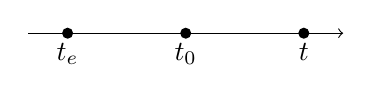
\begin{tikzpicture}
  \draw[->] (-2,0) -- (2,0);
  \node[below] at (-1.5,0) {$t_e$};
  \node[below] at (0,0) {$t_0$};
  \node[below] at (1.5,0) {$t$};
  \fill (-1.5,0) circle (2pt);
  \fill (0,0) circle (2pt);
  \fill (1.5,0) circle (2pt);
\end{tikzpicture}
\end{center}

The easiest way to calculate shifted distributions correctly is to start from the survival because ``the survival is multiplicative'' which means that surviving from start to finish is the same chance as surviving from start to a midpoint multiplied by the chance of surviving from midpoint to finish.
For a distribution shifted left, with midpoint $t_{0\alpha}$ and current time $t$,
\begin{equation}
	S_{\alpha}(t-t_{e\alpha}) = S_{\alpha}(t_{0\alpha} - t_{e\alpha})S_{\alpha}(t_{0\alpha}, t)
\end{equation}
Here, the $S$ with one argument is the survival function you would find in the Distributions package, and the $S$ with two arguments is the conditional survival written with absolute times as arguments. The equation above defines the conditional survival.
\begin{equation}
	S_{\alpha}(t_{0\alpha}, t) =  \frac{S_{\alpha}(t-t_{e\alpha})}{S_{\alpha}(t_{0\alpha} - t_{e\alpha})}
\end{equation}


\subsubsection{Right Shifted}

\begin{center}
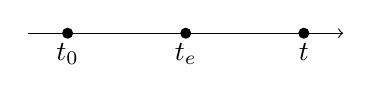
\begin{tikzpicture}
  \draw[->] (-2,0) -- (2,0);
  \node[below] at (-1.5,0) {$t_0$};
  \node[below] at (0,0) {$t_e$};
  \node[below] at (1.5,0) {$t$};
  \fill (-1.5,0) circle (2pt);
  \fill (0,0) circle (2pt);
  \fill (1.5,0) circle (2pt);
\end{tikzpicture}
\end{center}

For a distribution shifted right, that means the distribution can't fire until a certain time, so its survival is one until that time.
The conditional survival from $t_0$ to $t$ is just the survival,
\begin{equation}
  S_\alpha(t_0,t)=S_\alpha(t_0-t_e)
\end{equation}
There is a degenerate case where the time is less than the zero of the distribution, in which case, for $t<t_e$, $S(t_0,t)=1$.

We can unify the left shift and the right shift into one equation.
Use notation that $a\wedge b\coloneqq\mbox{min}(a,b)$ and $a\vee b\coloneqq\mbox{max}(a,b)$. Survival at time $t_e$ is always 1, by definition.
\begin{equation}
  S_\alpha(t_0,t)=\frac{S_\alpha((t-t_e)\vee 0)}{S_\alpha((t_0-t_e)\vee 0)}
\end{equation}
In each of the three cases, this simplifies to the correct equation given $t>t_0$, which is always the case.

\subsubsection{From Survival to Everything Else}

The hazard rate doesn't care about your shifts. It lives in the moment, counted since the zero of the distribution.
\begin{equation}
  \lambda(t_0, t, t_e) = \lambda(t-t_e)
\end{equation}
The CDF definitely cares but takes its cue from the survival.
\begin{equation}
 F(t_0,t,t_e) = 1-S(t_0,t,t_e) = 1-\frac{S_\alpha((t-t_e)\vee 0)}{S_\alpha((t_0-t_e)\vee 0)}
\end{equation}
This can be worked through.
\begin{eqnarray}
 F(t_0,t,t_e) & =& \frac{S_\alpha((t_0-t_e)\vee 0)-S_\alpha((t-t_e)\vee 0)}{S_\alpha((t_0-t_e)\vee 0)} \\
  & =& \frac{F_\alpha((t_0-t_e)\vee 0) - 1 -F_\alpha((t-t_e)\vee 0) + 1}{F_\alpha((t_0-t_e)\vee 0) - 1} \\
  & =& \frac{F_\alpha((t-t_e)\vee 0) - F_\alpha((t_0-t_e)\vee 0)}{1-F_\alpha((t_0-t_e)\vee 0)}
\end{eqnarray}
Remember that $S(0)=1$ so $F(0)=0$.

Lastly, the density of the CDF is the PDF. Most of the PDF terms are constant.
\begin{equation}
  f(t_0, t, t_e) = \frac{f_\alpha((t-t_e)\vee 0)}{1-F_\alpha((t_0-t_e)\vee 0)}=\frac{f_\alpha((t-t_e)\vee 0)}{S_\alpha((t_0-t_e)\vee 0)}
\end{equation}

\subsubsection{Likelihood with Shifted Distributions}

The survivals in Eq.~\ref{eqn:basic-likelihood} are conditional survivals starting at a last jump time $t_0$, and they are relative to enabling times. The hazard lives in the moment, so it doesn't care about some $t_0$ at the start of the time step, just about the distribution's definition of zero.
\begin{equation}
	c_{\alpha}(t|t_0) = \lambda_{\alpha}(t-t_{e\alpha})\prod_\beta S_{\beta}(t_0,t, t_{\beta e})\label{eqn:core-with-enabling}
\end{equation}
For a single time step from $t_0$ to $t$, the likelihood has one factor from the event that fires and then a factor from each event.
We saw above this can be rewritten into a pdf and survivals, which is more natural for the API in distributions.
\begin{equation}
	c_{\alpha}(t|t_0) = f_{\alpha}(t,t_0,t_{e\alpha})\prod_{\beta\ne\alpha} S_{\beta}(t_0,t, t_{\beta e})
\end{equation}
Using the replacements from above for time-shifting, and dropping the guards against negative durations, this becomes
\begin{equation}
	c_{\alpha}(t|t_0) = \frac{f_{\alpha}(t-t_{e\alpha})}{S_\alpha(t_{0\alpha}-t_{e\alpha})}\prod_{\beta\ne\alpha} \frac{S_{\beta}(t - t_{\beta e})}{S_\beta(t_{0\beta}-t_{e\beta})}
\end{equation}
The denominators in the two terms are the same but numerators are not. If we take the log of this, that affects what we sum over.
\begin{equation}
\ln c_{\alpha}(t|t_0) = \ln\:f_{\alpha}(t-t_{e\alpha})+\sum_{\beta\ne\alpha}\ln\:S_{\beta}(t - t_{\beta e}) - \sum_{\forall a}S_a(t_{0a}-t_{ea})
\end{equation}


For a trajectory consisting of multiple time steps, the likelihood is the product of all individual time steps. We know the product of conditional survivals, for the same event enabled over time, is equal to the conditional survival between the start and end times. It feels like we could use this to optimize our calculation.

Picture one transition, enabled at time $t_e$ and firing at time $t$. Its contribution to the likelihood of the whole trajectory would be just two factors. The function $f_\alpha$ is the pdf according to the Distributions package.
\begin{equation}
	\lambda_{\alpha}(t-t_{e\alpha})S_{\alpha}(t_0,t)
	=\lambda_{\alpha}(t-t_{e\alpha})\frac{S_{\alpha}(t-t_{e\alpha})}{S_{\alpha}((t_0-t_{e\alpha})\wedge 0)}
	=\frac{f_{\alpha}(t-t_{e\alpha})}{S_{\alpha}((t_0-t_{e\alpha})\wedge 0)}\label{eqn:event-lifetime-likelihood}
\end{equation}
If this transition were disabled without firing, it would contribute only the one factor, its conditional survival from enabling to disabling.

\subsection{Use Functions from Distributions Package}
Now that we know what math we want to calculate, let's look at which functions the Julia Distributions package offers. It doesn't give hazard rates, so we may prefer to work with the pdf, for instance. When the pdf is time-shifted, it complicates evaluation. Think about the log-likelihood for a single step, an incremental log-likelihood.
\begin{eqnarray}
	c_\alpha(t-t_0) &=& \lambda_\alpha(t-t_{e\alpha})S_\alpha(t_0,t,t_{e\alpha})\prod_{\beta\ne\alpha} S_\beta(t_0,t,t_{e\beta}) \\
	&=&
	\lambda_\alpha(t-t_{e\alpha})\frac{S_\alpha(t-t_{e\alpha})}{S_\alpha(t_0-t_{e\alpha})}\prod_{\beta\ne\alpha} S_\beta(t_0,t,t_{e\beta}) \\
	&=&
	\frac{f_\alpha(t-t_{e\alpha})}{S_\alpha(t_0-t_{e\alpha})}\prod_{\beta} S_\beta(t_0,t,t_{e\beta})
\end{eqnarray}

The log-likelihood of Eq.~\ref{eqn:core-with-enabling} becomes
\begin{equation}
  \log\:c_{\alpha}(t) = \log\:f_\alpha(t-t_{e\alpha})+\sum_{a\ne\alpha} \log\:S_a(t-t_{ea}) - \sum_{a\ne\alpha} \log\:S_a((t_t-t_{ea})\wedge 0).
\end{equation}
Note that the $S_\alpha$ in the denominator under $f_\alpha$ is removed from the product.
In Julia, there is a \texttt{logpdf}$\coloneqq\log\:f$ and a \texttt{logccdf}$\coloneqq\log\:S$.

There is also a version that uses integrated hazards\ldots

We can even more easily translate the log-likelihood associated with the lifetime of a single event, Eq.~\ref{eqn:event-lifetime-likelihood}.
\begin{equation}
	\log\:f_\alpha(t-t_{e\alpha}) - \log\:S_\alpha((t_0-t_{e\alpha})\wedge 0)
\end{equation}
That's for transitions that fired. For transitions that didn't fire, it's just the survival.
\begin{equation}
	\log\:S_\alpha(t-t_{e\alpha}) - \log\:S_\alpha((t_0-t_{e\alpha})\wedge 0)
\end{equation}
By summing these quantities over all events for every set of time periods the event is enabled, we can quickly get the likelihood of a trajectory.

\section{Gillespie's Direct Method}

We actually deal with the waiting time when using a Direct method. For a transition $a$ in the space of transitions $A$, the direct method breaks the marginal for next transition and time into a marginal for time and conditional for which transition fires at that time.
\begin{eqnarray*}
	P(A=a, t\le T_{n+1}-T_n<t+dt) &=& P(A=a|t\le T_{n+1}-T_n<t+dt) \\
	& & \qquad P(t\le T_{n+1}-T_n<t+dt)
\end{eqnarray*}
The last factor, $P(t\le T_{n+1}-T_n<t+dt)$, is the waiting time for the competing processes. In particular, the Direct method samples the waiting time using the usual method of inverting its survival with $u=P(\tau<T)$. In order to calculate the likelihood of a particular trajectory, we would need only to multiply $u$ by the hazard rate of the drawn transition.

We usually think of the direct method as sampling by inversion. If we write the direct method in terms of hazards a draw for time $T=\tau$, inversion sampling requires solving an inverse equation for the cumulative survival across competing processes.
\begin{equation}
	u = \mbox{exp}\left(-\int_{t_i}^\tau\sum_a \lambda_a(t)dt\right)
\end{equation}
There is, however, no reason that we can't use something like rejection sampling, where we sample in a two-dimensional space and keep samples that fall within the region under the density function. The efficiency of such rejection methods depends on choice of proposal distributions, so it's artful, but it should be much faster than direct integration.


\section{Common random numbers}

\subsection{Introduction}

Instead of calling \texttt{rand(rng, distribution)}, change it to \texttt{rand(rng, distribution, clock)}. Then keep track of a) the clock b) its $n$-th call and c) the survival associated with that call. Record choices and replay.

This works best with samplers that use fewer random numbers, such as the Next Reaction method. It's these lines we would want to replace. In the case of CRN, the input wouldn't be a random sample but would be a survival from which to determine the sample.

\begin{jllisting}
sample = rand(rng, distribution)
tau = te + sample
survival = survival_space(S, distribution, sample)
\end{jllisting}

What if you used CRN and a direct method? It doesn't seem like it would be very effective. Direct methods have two draws, one for the waiting time and one for the transition, conditional on the waiting time draw. I could see this working if the transitions were ordered in a meaningful way. The draw for which transition fires is a discrete choice, found by inverting this to find the largest transition $\alpha$ for which
\begin{equation}
	u \le \sum_{0}^{\alpha}\lambda_i(t).
\end{equation}
Subsequent runs of the simulation would pick values with the same $u$, and if nearby values were meaningfully similar, that would be an interesting constraint.

\subsection{Julia Implementation}

In Julia, when you draw from a distribution, it constructs a Sampler for that distribution. For instance, if a Gamma distribution is most easily sampled with one sampler for typical parameters and another sampler for smaller shape values. The sampler for the distribution will rely on capabilities of the random number generator and may construct a second type of Sampler for the random number generator. For instance, it may choose to draw 128-bit unsigned integers or it may choose to draw doubles. Julia's sampling architecture is therefore highly configurable for optimization.

CRN traditionally stores a draw from a uniform variate, and that's it. It assumes you will sample by inversion. We could do that, or we could hook into Julia's system in more depth. Let's list some possibilities, not in order of preference but numbered for reference.
\begin{enumerate}
	\item Save a uniform variate.
	\item Save the state of the random number generator, either to support multiple draws or support draws of specific values, such as 128-bit unsigned integers. The state of the Xoshiro generator is only 256 bits of storage, and linear congruential generators can have very small state, but Mersenne twister state is much, much larger.
	\item Figure out which particular values are drawn from the RNG and save those.
\end{enumerate}
Maybe we could try both the first and second options.

The random variates need to be stored in order to reuse them. We already have the notion of a clock ID, so we're storing a value for each (clock ID, ordinal). A simulation may have only one clock and a million calls, or it may have a million clocks called once each. We won't know going into a run which one will happen, so I suppose it would make sense to record everything in some simple way and then repack it for replaying later.


\section{Importance Sampling}

Why would you calculate a likelihood? So that you can artificially increase the likelihood of trajectories with desired outcomes in order to improve their statistics.

For a simulation with a likelihood $f_a(t)$, the importance sampling technique samples instead from a likelihood $g_a(t)$. We weight the ensuing trajectory by $f_a(t)/g_a(t)$. The likelihood ratio consists of quantities we've already discussed calculating.
\begin{equation}
	\frac{f_a(t)}{g_a(t)} = \frac{\lambda_{\alpha}(t)\prod_{a}S_a(t)}{\lambda'_{\alpha}(t)\prod_{b}S'_b(t)}\label{eqn:likelihoodratio}
\end{equation}
If we can draw from $g$, then we only need to calculate hazards and survivals, or pdf and survivals, to calculate the ratio.

We have our three basic ways to draw: transition first, time first, or competing processes.
\begin{eqnarray}
	P[A,T]&=&P[A]P[T|A]\qquad\mbox{(nobody)} \\
	&=&P[A|T]P[T]\qquad\mbox{(direct)}\\
	&=&\mbox{min}(P[T_a])\ \forall a\qquad\mbox{(competing)}
\end{eqnarray}
We know what those pieces are, too, and the first equation explains why nobody draws the transition first, then the time given the transition.
\begin{eqnarray}
	P[A] & = & \int_{t_0}^\infty \lambda_{\alpha}(t)\prod_{a}S_a(t)dt\label{eqn:marginaltransition} \\
	P[t\le T<t+dt|A] & = & \lambda_{\alpha}(t)\prod_{a}S_a(t)dt \\
	P[A|T] & = & \frac{\lambda_\alpha(t)}{\sum_a\lambda_a(t)} \\
	P[T] & = & 1-\exp(-\sum_a\int_{t_0}^t\lambda_a(s)ds) \\
	P[T_a] & = & 1-\exp(-\int_{t_0}^t \lambda_a(s)ds)
\end{eqnarray}
The good news is that there is no reason to calculate Eq.~\ref{eqn:marginaltransition} in order to use importance sampling. We can draw from some $g$ and then evaluate the likelihood of the draw for both the proposal distribution and the target distribution.


\subsection{Splitting}

This version of importance sampling is simple to implement. When a trajectory is in the right direction, split it into multiple trajectories. Then, when counting results, down-weight those trajectories by the split. If one trajectory splits into 10, count the results by 1/10th.

A good example of splitting is a simulation that takes place on an energy landscape. Picture two valleys and a mountain pass between them. The simulation starts in one valley and rarely crosses the pass to the next valley. For those simulations that approach the pass, you could split the trajectories in order to increase the quality of statistics for the likelihood of reaching the other valley.

Splitting is implemented not in the sampler but in the driver of the simulation. You would copy the simulation state and the sampler state $N$ times and then down-weight the contribution of each.

For someone who wants to use this kind of splitting, they will define a trigger for splitting. This is a stopping time where the simulation is at or near a desired set of outcomes. It's a condition on the state of the simulation, not a condition on the sampler. The act of splitting creates multiple trajectories, each with its own sampler. CompetingClocks can support this by making it easy to copy a sampler so that a simulation can spawn a new trajectory. These new trajectories may run simultaneously or one after the other, but that wouldn't matter as long as the system state and samplers were separate copies.


\subsection{Exclusion}

Here, we choose a transition and disallow it from firing. For instance, it's common in disease modeling to ask how large an outbreak would be, were there an outbreak. That's a conditional probability, conditioned on the disease never reaching extinction. 

There are two ways to calculate an exclusion-sampled trajectory. Picture a herd of animals with only one infectious. It could either recover or infect another in the herd, and we'll exclude recovery, but we have to account for the decreased likelihood of the trajectory given that it excludes recovery.

Let's say there are two transitions, A for 1/3 of the time, B for 1/3 of the time, C for 1/3 of the time. We exclude A, so B goes all the time. We should reweight B's and C's trajectories by 2/3.

If we go back to Eq.~\ref{eqn:likelihoodratio}, then importance sampling with exclusion leaves out one survival. Call that $A=\beta$.
\begin{equation}
	\frac{f_\alpha(t)}{g_\alpha(t)} = \frac{\lambda_{\alpha}(t)S_\beta(t)\prod_{a}S_a(t)}{\lambda_{\alpha}(t)\prod_{a}S_a(t)} = S_\beta(t)
\end{equation}
The algorithm then is to keep the transition you want to exclude updated, as with any other transition.
\begin{enumerate}
	\item Draw from all transitions except the excluded one. Ignore it.
	\item Calculate the survival of the excluded transition.
	\item Weight the ensuing trajectory by the survival of the excluded transition.
\end{enumerate}
In other words, you're weighting the trajectory by the probability the excluded transition would already have fired.

\subsection{Weighting Probability}

We could implement a simulation where all of the individual distribution functions differ from the target functions. At each step, we would reweight the trajectory likelihood. You would have to keep two samplers around, one to calculate likelihood of the target distributions and one to both draw from and calculate likelihood of proposal distributions.

\subsection{Tools for Importance Sampling}

The hardest part of importance sampling is figuring out how to make the estimates better and not worse. You need to calculate the change in variance of estimates with and without importance sampling. We might need to think about tooling to help calculate the best weights to use.


\subsection{Examples}
Example: Preventing extinction in disease simulation.

Example: Estimation of energy barrier.


\section{Hamiltonian Monte Carlo}

My favorite housing spread example.


\section{Piecewise Deterministic Markov Processes}

As long as the sampler can sample the distribution using the given methods, that distribution can be determined by any equation, including an ODE. In one version, the distribution is a delta function, and these completely work. You have to re-enable the distribution each time the ODE changes its prediction. In another version, there is still a continuous distribution, but it's determined by the ODE.

Show that a delta-function can be included in CompetingClocks.

\end{document}
